\documentclass[11pt,a4paper]{article}
\usepackage[margin=2.3cm]{geometry}
\usepackage{amsmath,amssymb}
\usepackage{graphicx}
\usepackage{epstopdf}          % converts the .eps figures automatically when compiling with pdflatex
\usepackage{booktabs}
\usepackage{multirow}
\usepackage{float}
\usepackage{caption}
\usepackage[dvipsnames]{xcolor}
\usepackage{tikz}
\usetikzlibrary{positioning,arrows.meta,fit,backgrounds}
\usepackage[colorlinks=true,linkcolor=blue!50!black,citecolor=blue!50!black,urlcolor=blue!50!black]{hyperref}
\graphicspath{{figures/}}

\title{\textbf{Glucose--Insulin Dynamics in Type 1 Diabetes:\\ the Bergman Minimal Model and a Hybrid Universal Neural ODE}}
\author{Leora Modi (2023B4AD0866G), Saee Brahmankar (2023B4AD0909G), Meghana Mahesh (2023B1AD0682G), Prateek Singhal (2024ADPS0830G), Atharva Sawant (2024ADPS0872G)} \textcolor{red}}
\date{Mathematical Modelling -- Group Project, November 2026}

\begin{document}
\maketitle

\begin{abstract}
People with Type 1 diabetes make no insulin and must decide, several times a day, how much to inject for the food they eat. We model this with the Bergman minimal model, adapted to Type 1 diabetes by removing pancreatic secretion and adding subcutaneous insulin absorption and a gut compartment. We derive the equilibrium under basal insulin in closed form and prove it is a locally asymptotically stable node; we study parameter identifiability and local and global (Sobol) sensitivity; and we verify first-order convergence of the numerical scheme. As an extension, we replace the gut transfer rates with small mass-conserving neural networks inside the ODE (a universal differential equation, UDE), trained by back-propagation through the solver. On ten virtual patients from the UVA/Padova simulator, where the true meal absorption is known, the hybrid model rediscovers a hidden nonlinear gut law from glucose data alone in a twin experiment (meal-appearance error 41\% $\to$ 7\%, forecast RMSE 14.4 $\to$ 6.1\,mg/dL), and modestly improves forecasts on the misspecified UVA/Padova simulator (10.9 $\to$ 10.2\,mg/dL). On real free-living data from 15 patients (HUPA-UCM dataset), we compare 4-hour forecasts on held-out days and on patients unseen in training against persistence and an LSTM: the physiology-based models beat persistence and the LSTM on held-out days (RMSE 42.7 hybrid, 43.1 Bergman, 48.5 LSTM, 49.8\,mg/dL persistence), and on unseen patients the hybrid improves on Bergman by 8\%. Unlogged meals and exercise keep absolute errors large.
\end{abstract}

\section{Introduction and motivation}
Type 1 diabetes is an autoimmune disease that destroys the insulin-producing $\beta$-cells of the pancreas. Patients replace insulin by injections or a pump and measure glucose with a continuous glucose monitor (CGM). Too little insulin leads to hyperglycaemia and long-term organ damage; too much leads to hypoglycaemia, which can be dangerous within minutes. Every meal therefore poses a prediction problem: \emph{given this meal and this dose, where will my glucose be in the next few hours?} Mathematical models of the glucose--insulin system are the basis of insulin dose calculators and of the artificial pancreas.

The Bergman minimal model \cite{bergman1979} is the classic compact description of glucose--insulin interaction. It is interpretable --- each parameter has a physiological meaning --- but describes the absorption of a meal from the gut only crudely. Machine-learning forecasters can be flexible but are black boxes that need much data and can violate physical laws. \emph{Universal differential equations} \cite{rackauckas2020} combine the two: known mechanisms stay as equations and a neural network learns only the unknown part.

\paragraph{Objectives.}
\begin{enumerate}
  \item Formulate a Bergman-type model for Type 1 diabetes driven by recorded insulin and meals.
  \item Analyse it: equilibrium, stability, identifiability, local and global sensitivity, and numerical convergence.
  \item Fit it to real patients and assess its forecasts on data not used for fitting.
  \item Extend it with a hybrid UDE that learns gut absorption, validate this where the truth is known (simulator), and compare it with the mechanistic model, a persistence forecast and an LSTM.
\end{enumerate}

\section{Data}
\paragraph{Real patients.} The HUPA-UCM dataset \cite{hupa2024} contains CGM glucose (FreeStyle Libre 2), insulin (basal and bolus) and logged carbohydrate for 25 people with Type 1 diabetes, at 5-minute resolution, for at least 14 days each. Profiling all files showed: (i) carbohydrate is logged in 10\,g portions by most patients but in grams by three; (ii) seven patients lack insulin or meal records, or log them only as constant markers; (iii) two patients' glucose is more than half straight-line gap fill. After exclusions, 15 patients remain (Table~\ref{tab:cohort}). The CGM is a 15-minute sensor linearly interpolated to 5 minutes; straight-line stretches of 30 minutes or more (filled sensor gaps) and readings at the 40\,mg/dL sensor floor are masked out of every fit and error metric. Records longer than 30 days are cut to the 30-day block with the most complete basal-insulin record.

\paragraph{Meal windows and test design.} A forecasting window is the 4 hours after a logged meal, kept only if no meal was logged in the preceding 3 hours, basal insulin was recorded for at least 95\% of the preceding 6 hours and the window, and at least 80\% of the window's readings are valid. For each patient, windows in the first 70\% of days are used for fitting (the last 20\% of these for validation/early stopping) and windows in the last 30\% for testing. Four patients (0005, 0016, 0017, 0024) are additionally kept out of neural-network training altogether. This gives 227 fitting, 64 validation and 112 test windows.

\begin{table}[H]
\centering
\caption{Patients used (HUPA-UCM). Excluded: 0009 (100\% of glucose is gap-filled); 0010 (90\% of glucose is gap-filled); 0011 (no insulin); 0014 (no basal record); 0015 (no insulin, no meals); 0018 (no insulin, no meals); 0019 (meals/boluses only as 1-markers); 0020 (no meals); 0021 (meals/boluses only as 1-markers); 0026 (only 0 usable meal windows for fitting). Mean glucose in mg/dL; masked = gap-filled or sensor-floor readings.}
\label{tab:cohort}
\small
\begin{tabular}{lllrrlr}
\toprule
 & days & carb unit & meals/day & insulin U/day & mean glucose & masked \% \\
Patient &  &  &  &  &  &  \\
\midrule
0001 & 14 & 10 g & 2.8 & 25.4 & 181 & 2.4 \\
0002 & 11 & g & 1.1 & 46.5 & 113 & 8.5 \\
0003 & 13 & 10 g & 5.0 & 36.2 & 143 & 1.8 \\
0004 & 11 & g & 1.8 & 64.0 & 180 & 16.5 \\
0005 & 13 & 10 g & 4.1 & 26.7 & 148 & 2.1 \\
0006 & 8 & 10 g & 4.7 & 50.2 & 165 & 5.6 \\
0007 & 13 & 10 g & 6.1 & 58.4 & 173 & 2.2 \\
0016 & 13 & 10 g & 6.2 & 40.4 & 150 & 15.0 \\
0017 & 12 & 10 g & 2.8 & 22.4 & 201 & 8.3 \\
0022 & 14 & g & 4.9 & 66.9 & 113 & 7.8 \\
0023 & 14 & 10 g & 4.6 & 20.5 & 133 & 0.9 \\
0024 & 10 & 10 g & 1.4 & 19.0 & 167 & 2.4 \\
0025 & 14 & 10 g & 1.4 & 53.1 & 114 & 4.6 \\
0027 & 30 & 10 g & 3.7 & 45.8 & 118 & 5.9 \\
0028 & 30 & 10 g & 4.0 & 23.4 & 128 & 11.7 \\
\bottomrule
\end{tabular}
\end{table}


\paragraph{Virtual patients.} Ten virtual adults were simulated for 14 days each with the UVA/Padova Type 1 simulator \cite{dallaman2007,kovatchev2009} (Python implementation \texttt{simglucose} \cite{simglucose}), with three meals a day and occasional snacks, standard basal--bolus therapy, and CGM noise of SD 5\,mg/dL. The simulator records the true rate of glucose appearance from the gut, which is never observable in real patients.

\section{Assumptions}
\begin{enumerate}
  \item Glucose kinetics are described by a single plasma compartment (Bergman); interstitial CGM glucose equals plasma glucose (the 5--10\,min sensor lag is neglected).
  \item Type 1 diabetes: no endogenous insulin secretion; all plasma insulin comes from recorded basal and bolus doses.
  \item Subcutaneous insulin absorption follows a two-compartment linear chain with population constants \cite{hovorka2004}.
  \item Meals are logged at the time they are eaten with the logged carbohydrate amount, and are absorbed through a two-compartment gut.
  \item Body weight (not in the data) is 70\,kg; it rescales $S_I$ and the meal effect, which the fitted parameters absorb.
  \item Within a 4-hour window, patient parameters are constant (no exercise, illness or circadian effects).
\end{enumerate}

\section{Mathematical formulation}
Figure~\ref{fig:diagram} shows the model structure.
\begin{figure}[H]
\centering
\resizebox{\textwidth}{!}{% Compartment diagram of the model. Included in report.tex with % Compartment diagram of the model. Included in report.tex with % Compartment diagram of the model. Included in report.tex with \input{diagrams/compartment_diagram.tex}
% (needs \usepackage{tikz} and \usetikzlibrary{positioning,arrows.meta,fit,backgrounds}).
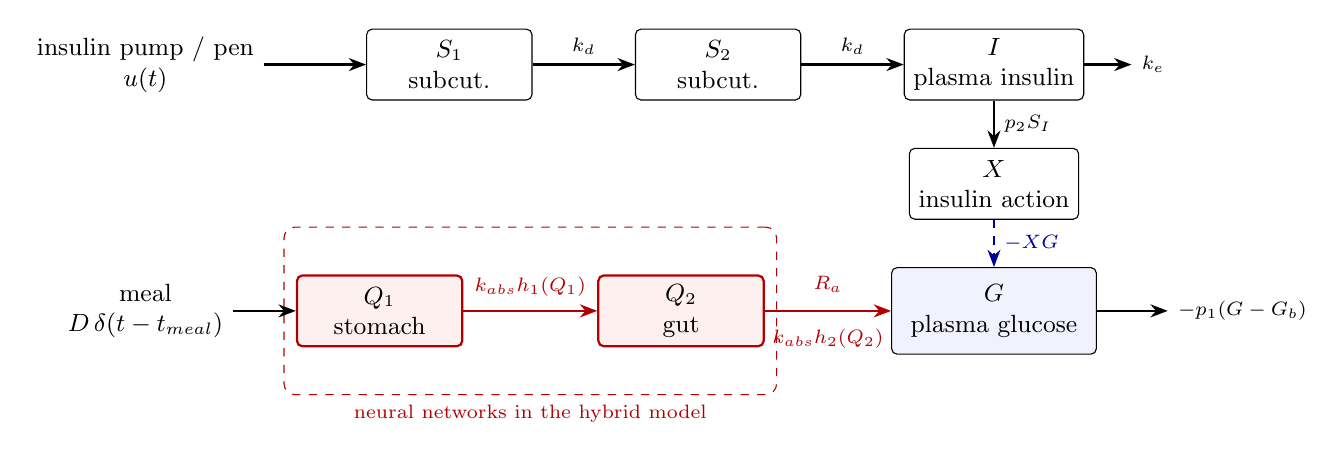
\begin{tikzpicture}[
    node distance=6mm and 13mm,
    box/.style={draw, rounded corners=2pt, minimum width=21mm, minimum height=9mm, align=center, font=\small, fill=white},
    nn/.style={box, draw=red!70!black, thick, fill=red!6},
    inp/.style={font=\small, align=center},
    flow/.style={-{Stealth[length=2.2mm]}, thick},
    act/.style={-{Stealth[length=2.2mm]}, thick, dashed, blue!60!black}
]
  % insulin chain
  \node[inp] (u) {insulin pump / pen\\ $u(t)$};
  \node[box, right=of u] (s1) {$S_1$\\ subcut.};
  \node[box, right=of s1] (s2) {$S_2$\\ subcut.};
  \node[box, right=of s2] (I) {$I$\\ plasma insulin};
  \node[box, below=of I] (X) {$X$\\ insulin action};
  % glucose
  \node[box, below=of X, minimum width=26mm, minimum height=11mm, fill=blue!5] (G) {$G$\\ plasma glucose};
  % gut chain
  \node[inp] (D) at (u |- G) {meal\\ $D\,\delta(t-t_{meal})$};
  \node[nn, right=8mm of D] (q1) {$Q_1$\\ stomach};
  \node[nn, right=17mm of q1] (q2) {$Q_2$\\ gut};

  \draw[flow] (u) -- (s1);
  \draw[flow] (s1) -- node[above, font=\scriptsize] {$k_d$} (s2);
  \draw[flow] (s2) -- node[above, font=\scriptsize] {$k_d$} (I);
  \draw[flow] (I) -- node[right, font=\scriptsize] {$p_2 S_I$} (X);
  \draw[flow] (I.east) -- ++(6mm,0) node[right, font=\scriptsize] {$k_e$};
  \draw[act] (X) -- node[right, font=\scriptsize] {$-X G$} (G);
  \draw[flow] (D) -- (q1);
  \draw[flow, red!70!black] (q1) -- node[above=0.5mm, font=\scriptsize] {$k_{abs}h_1(Q_1)$} (q2);
  \draw[flow, red!70!black] (q2) -- node[above=1mm, font=\scriptsize] {$R_a$} node[below=1mm, font=\scriptsize] {$k_{abs}h_2(Q_2)$} (G);
  \draw[flow] (G.east) -- ++(9mm,0) node[right, font=\scriptsize, align=left] {$-p_1(G-G_b)$};

  \begin{scope}[on background layer]
    \node[draw=red!70!black, dashed, rounded corners, fit=(q1)(q2), inner xsep=1.5mm, inner ysep=6mm,
          label={[font=\scriptsize, red!70!black]below:neural networks in the hybrid model}] {};
  \end{scope}
\end{tikzpicture}

% (needs \usepackage{tikz} and \usetikzlibrary{positioning,arrows.meta,fit,backgrounds}).
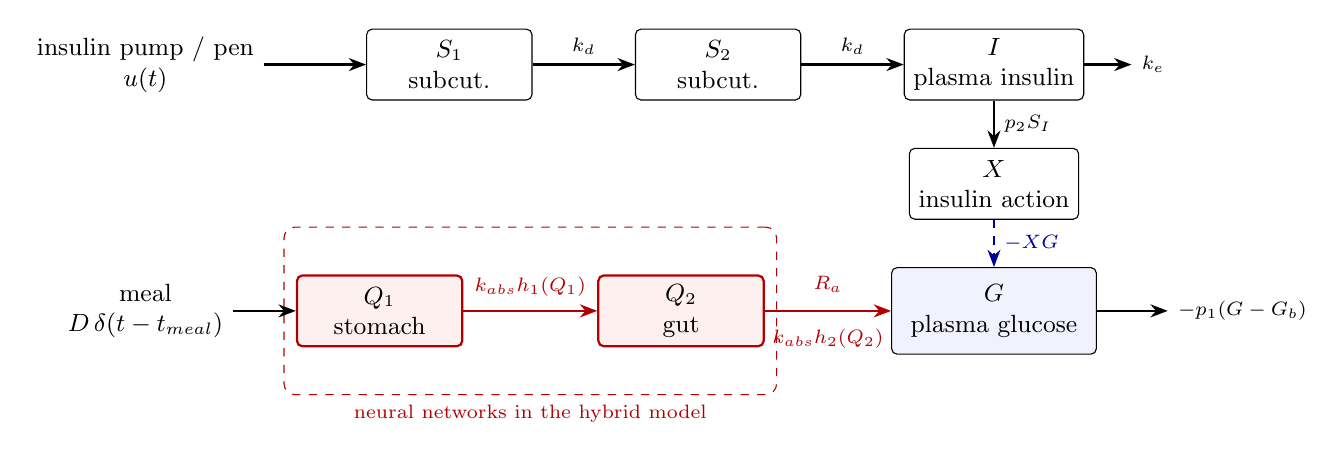
\begin{tikzpicture}[
    node distance=6mm and 13mm,
    box/.style={draw, rounded corners=2pt, minimum width=21mm, minimum height=9mm, align=center, font=\small, fill=white},
    nn/.style={box, draw=red!70!black, thick, fill=red!6},
    inp/.style={font=\small, align=center},
    flow/.style={-{Stealth[length=2.2mm]}, thick},
    act/.style={-{Stealth[length=2.2mm]}, thick, dashed, blue!60!black}
]
  % insulin chain
  \node[inp] (u) {insulin pump / pen\\ $u(t)$};
  \node[box, right=of u] (s1) {$S_1$\\ subcut.};
  \node[box, right=of s1] (s2) {$S_2$\\ subcut.};
  \node[box, right=of s2] (I) {$I$\\ plasma insulin};
  \node[box, below=of I] (X) {$X$\\ insulin action};
  % glucose
  \node[box, below=of X, minimum width=26mm, minimum height=11mm, fill=blue!5] (G) {$G$\\ plasma glucose};
  % gut chain
  \node[inp] (D) at (u |- G) {meal\\ $D\,\delta(t-t_{meal})$};
  \node[nn, right=8mm of D] (q1) {$Q_1$\\ stomach};
  \node[nn, right=17mm of q1] (q2) {$Q_2$\\ gut};

  \draw[flow] (u) -- (s1);
  \draw[flow] (s1) -- node[above, font=\scriptsize] {$k_d$} (s2);
  \draw[flow] (s2) -- node[above, font=\scriptsize] {$k_d$} (I);
  \draw[flow] (I) -- node[right, font=\scriptsize] {$p_2 S_I$} (X);
  \draw[flow] (I.east) -- ++(6mm,0) node[right, font=\scriptsize] {$k_e$};
  \draw[act] (X) -- node[right, font=\scriptsize] {$-X G$} (G);
  \draw[flow] (D) -- (q1);
  \draw[flow, red!70!black] (q1) -- node[above=0.5mm, font=\scriptsize] {$k_{abs}h_1(Q_1)$} (q2);
  \draw[flow, red!70!black] (q2) -- node[above=1mm, font=\scriptsize] {$R_a$} node[below=1mm, font=\scriptsize] {$k_{abs}h_2(Q_2)$} (G);
  \draw[flow] (G.east) -- ++(9mm,0) node[right, font=\scriptsize, align=left] {$-p_1(G-G_b)$};

  \begin{scope}[on background layer]
    \node[draw=red!70!black, dashed, rounded corners, fit=(q1)(q2), inner xsep=1.5mm, inner ysep=6mm,
          label={[font=\scriptsize, red!70!black]below:neural networks in the hybrid model}] {};
  \end{scope}
\end{tikzpicture}

% (needs \usepackage{tikz} and \usetikzlibrary{positioning,arrows.meta,fit,backgrounds}).
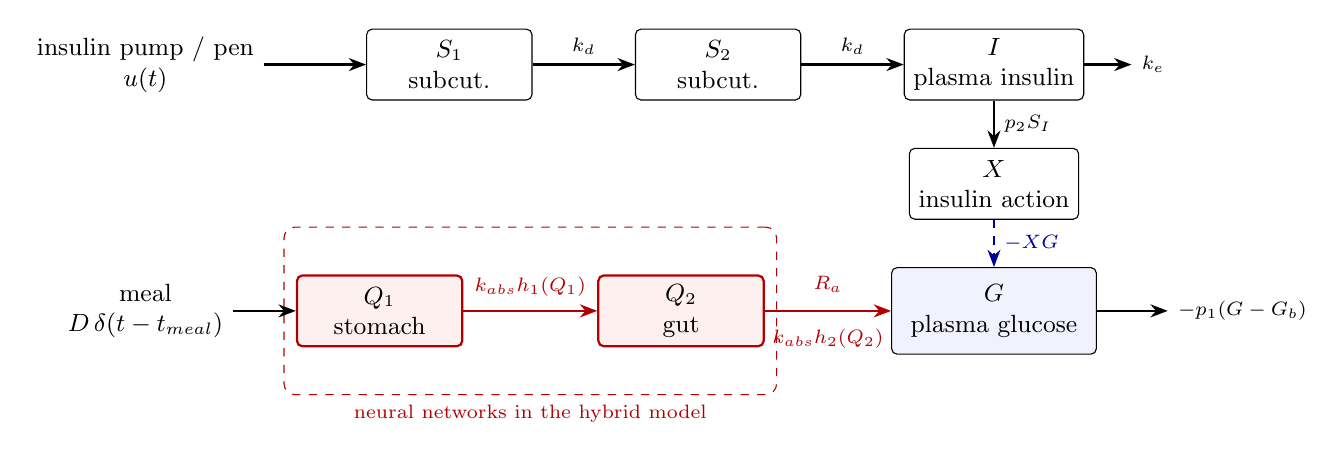
\begin{tikzpicture}[
    node distance=6mm and 13mm,
    box/.style={draw, rounded corners=2pt, minimum width=21mm, minimum height=9mm, align=center, font=\small, fill=white},
    nn/.style={box, draw=red!70!black, thick, fill=red!6},
    inp/.style={font=\small, align=center},
    flow/.style={-{Stealth[length=2.2mm]}, thick},
    act/.style={-{Stealth[length=2.2mm]}, thick, dashed, blue!60!black}
]
  % insulin chain
  \node[inp] (u) {insulin pump / pen\\ $u(t)$};
  \node[box, right=of u] (s1) {$S_1$\\ subcut.};
  \node[box, right=of s1] (s2) {$S_2$\\ subcut.};
  \node[box, right=of s2] (I) {$I$\\ plasma insulin};
  \node[box, below=of I] (X) {$X$\\ insulin action};
  % glucose
  \node[box, below=of X, minimum width=26mm, minimum height=11mm, fill=blue!5] (G) {$G$\\ plasma glucose};
  % gut chain
  \node[inp] (D) at (u |- G) {meal\\ $D\,\delta(t-t_{meal})$};
  \node[nn, right=8mm of D] (q1) {$Q_1$\\ stomach};
  \node[nn, right=17mm of q1] (q2) {$Q_2$\\ gut};

  \draw[flow] (u) -- (s1);
  \draw[flow] (s1) -- node[above, font=\scriptsize] {$k_d$} (s2);
  \draw[flow] (s2) -- node[above, font=\scriptsize] {$k_d$} (I);
  \draw[flow] (I) -- node[right, font=\scriptsize] {$p_2 S_I$} (X);
  \draw[flow] (I.east) -- ++(6mm,0) node[right, font=\scriptsize] {$k_e$};
  \draw[act] (X) -- node[right, font=\scriptsize] {$-X G$} (G);
  \draw[flow] (D) -- (q1);
  \draw[flow, red!70!black] (q1) -- node[above=0.5mm, font=\scriptsize] {$k_{abs}h_1(Q_1)$} (q2);
  \draw[flow, red!70!black] (q2) -- node[above=1mm, font=\scriptsize] {$R_a$} node[below=1mm, font=\scriptsize] {$k_{abs}h_2(Q_2)$} (G);
  \draw[flow] (G.east) -- ++(9mm,0) node[right, font=\scriptsize, align=left] {$-p_1(G-G_b)$};

  \begin{scope}[on background layer]
    \node[draw=red!70!black, dashed, rounded corners, fit=(q1)(q2), inner xsep=1.5mm, inner ysep=6mm,
          label={[font=\scriptsize, red!70!black]below:neural networks in the hybrid model}] {};
  \end{scope}
\end{tikzpicture}
}
\caption{Compartment diagram. Black: insulin absorption and action; blue: glucose; red: gut, whose transfer rates are neural networks in the hybrid model.}
\label{fig:diagram}
\end{figure}

\paragraph{Insulin absorption.} With insulin input $u(t)$ (mU/min),
\begin{equation}
\dot S_1 = u - k_d S_1,\qquad \dot S_2 = k_d(S_1-S_2),\qquad \dot I = \frac{k_d S_2}{V_I\,BW} - k_e I .
\label{eq:insulin}
\end{equation}
\paragraph{Gut absorption.} A meal of $D$ mg eaten at $t_m$ enters the stomach $Q_1$, then the gut $Q_2$, and appears in plasma at rate $R_a$ (mg/kg/min):
\begin{equation}
\dot Q_1 = D\,\delta(t-t_m) - k_{abs} Q_1,\qquad \dot Q_2 = k_{abs}(Q_1-Q_2),\qquad R_a = \frac{f\,k_{abs}\,Q_2}{BW}.
\label{eq:gut}
\end{equation}
\paragraph{Glucose--insulin interaction (Bergman, Type 1).}
\begin{equation}
\dot G = -p_1 (G-G_b) - X G + \frac{R_a}{V_G},\qquad \dot X = -p_2 X + p_2 S_I\, I .
\label{eq:bergman}
\end{equation}
Here $G$ is plasma glucose (mg/dL), $X$ the remote insulin action (min$^{-1}$), $p_1$ glucose effectiveness, $p_2$ the rate at which insulin action builds up and decays, $S_I$ insulin sensitivity ($p_3=p_2S_I$ in Bergman's notation) and $G_b$ the level towards which non-insulin mechanisms drive glucose. Fixed constants \cite{hovorka2004,dallaman2007}: $k_d=0.018$, $k_e=0.138$\,min$^{-1}$, $V_I=0.12$\,L/kg, $V_G=1.6$\,dL/kg, $f=0.9$, $BW=70$\,kg. Fitted per patient: $\theta=(p_1,p_2,S_I,G_b,k_{abs})$.

\section{Mathematical analysis}
\subsection{Equilibrium under basal insulin}
With no meal and constant basal infusion $u_b$, setting \eqref{eq:insulin}--\eqref{eq:bergman} to zero gives successively
\begin{equation}
S_1^*=S_2^*=\frac{u_b}{k_d},\quad I^*=\frac{u_b}{k_e V_I BW},\quad X^*=S_I I^*,\quad Q_1^*=Q_2^*=0,\quad G^*=\frac{p_1 G_b}{p_1+S_I I^*}.
\label{eq:eq}
\end{equation}
The equilibrium exists and is unique for all positive parameters. Fasting glucose $G^*$ falls monotonically as basal insulin $u_b$ or insulin sensitivity $S_I$ rises, and $\partial G^*/\partial u_b = -G^* S_I/(k_eV_IBW(p_1+X^*))$ quantifies how a basal-rate change moves fasting glucose.

\subsection{Local stability}
\textbf{Proposition.} The equilibrium \eqref{eq:eq} is locally asymptotically stable; it is a stable node (no oscillation).

\textit{Proof.} Order the state as $y=(S_1,S_2,I,Q_1,Q_2,X,G)$. Each variable depends only on itself and on variables earlier in this list (insulin and gut are autonomous linear chains; $X$ depends on $I$; $G$ on $X$, $Q_2$ and itself). The Jacobian at $y^*$ is therefore lower triangular, and its eigenvalues are its diagonal entries
\[
\lambda\in\{-k_d,\,-k_d,\,-k_e,\,-k_{abs},\,-k_{abs},\,-p_2,\,-(p_1+X^*)\},
\]
which are real and strictly negative. By the Hartman--Grobman theorem the nonlinear system is locally asymptotically stable, and real eigenvalues mean trajectories approach without oscillation. $\square$

The slowest return rate, $\min(p_2,\,p_1+X^*,\,k_{abs})$, sets how long a disturbance persists. We confirmed the result numerically for every fitted patient by computing the Jacobian with automatic differentiation: all eigenvalues are real and negative (largest: $-0.0013$\,min$^{-1}$). Figure~\ref{fig:phase} shows trajectories in the $(G,X)$ plane converging to the node.

\begin{figure}[H]
\centering
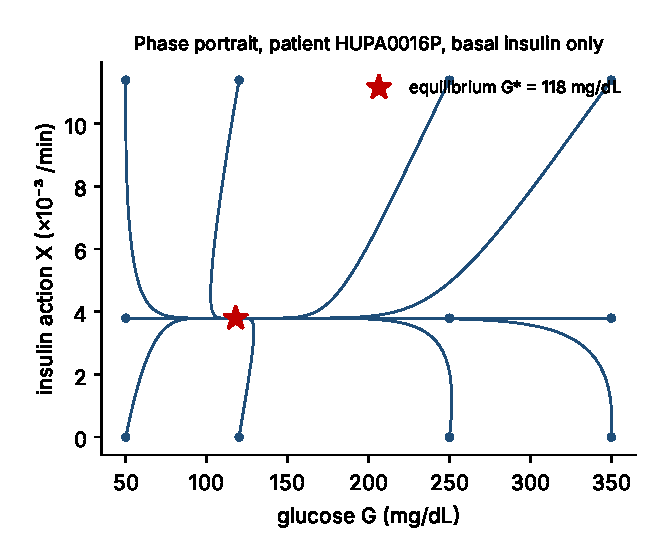
\includegraphics[width=0.55\textwidth]{phase_portrait.eps}
\caption{Phase portrait for the reference patient (HUPA0016P, fitted parameters, own basal rate 0.88\,U/h): from any starting glucose and insulin action, trajectories converge to the equilibrium without oscillating.}
\label{fig:phase}
\end{figure}

\subsection{Parameter estimation and identifiability}
For each patient, $\hat\theta$ minimises the mean squared error between simulated and observed glucose over that patient's training windows (valid readings only). Parameters are mapped into physiological bounds by a sigmoid in log-space, and gradients are obtained by automatic differentiation through the solver (PyTorch) and used by the Adam optimiser. Each patient is fitted from 6 random starts.

Identifiability was checked in two ways (Table~\ref{tab:ident}, Figure~\ref{fig:ident}): the spread of parameters among starts reaching the same error, and the local covariance $\mathrm{Cov}(\log\hat\theta)\approx\hat\sigma^2(J^\top J)^{-1}$ from the sensitivity matrix $J_{ij}=\partial r_i/\partial\log\theta_j$. Multi-start fits agree closely (median spread 3--11\\%), so the optimiser reliably finds the same minimum; but the local analysis shows that $p_2$, $p_1$ and $G_b$ have large relative standard errors (67\%, 49\% and 44\%) and $p_1$, $S_I$, $G_b$ are mutually correlated. $S_I$ and $k_{abs}$ are best determined. The fitted values are therefore effective parameters rather than clinical measurements.

\begin{table}[H]
\centering
\caption{Identifiability of the fitted parameters (medians over patients).}
\label{tab:ident}
\small
\begin{tabular}{lrr}
\toprule
 & multi-start CV (median) & relative SE (median) \\
\midrule
$p_1$ & 0.11 & 0.49 \\
$p_2$ & 0.03 & 0.67 \\
$S_I$ & 0.04 & 0.20 \\
$G_b$ & 0.05 & 0.44 \\
$k_{abs}$ & 0.03 & 0.12 \\
\bottomrule
\end{tabular}
\end{table}


\begin{figure}[H]
\centering
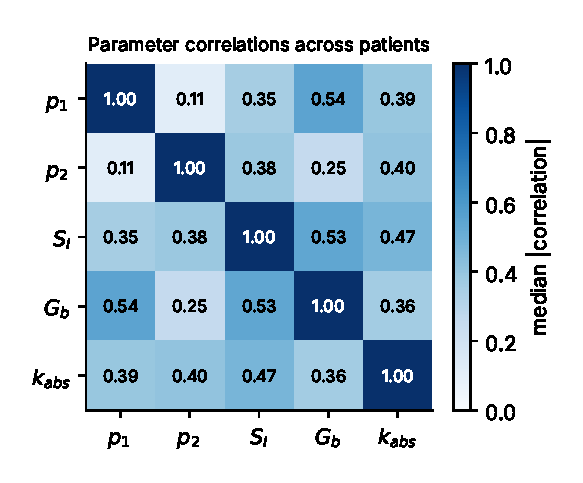
\includegraphics[width=0.45\textwidth]{identifiability_corr.eps}
\caption{Median absolute correlation between parameter estimates across patients. Strongly correlated pairs can compensate for each other and are hard to estimate separately.}
\label{fig:ident}
\end{figure}

\subsection{Sensitivity analysis}
For a reference patient --- the one whose fitted fasting equilibrium is closest to 120\,mg/dL --- receiving a 50\,g meal with a 5\,U bolus, the normalised local sensitivity $S_{\theta_i}(t)=\frac{\theta_i}{G}\frac{\partial G}{\partial\theta_i}$ (Figure~\ref{fig:sens}, left) shows how a 1\% change in each parameter changes glucose over time. For a global view, all five parameters were varied together, log-uniformly between half and double the reference patient's values, and Sobol variance-based indices \cite{saltelli2002,salib} were estimated from 12\,288 simulations (Figure~\ref{fig:sens}, right; Table~\ref{tab:sobol}). Reference patient 0016 (fasting equilibrium 118\,mg/dL on 0.88\,U/h basal). Insulin sensitivity $S_I$ and $G_b$ together explain about two thirds of the variance of peak and 2-hour glucose, followed by $p_1$; $p_2$ has essentially no influence. This explains the identifiability result: a parameter the output barely depends on cannot be estimated from that output.

\begin{figure}[H]
\centering
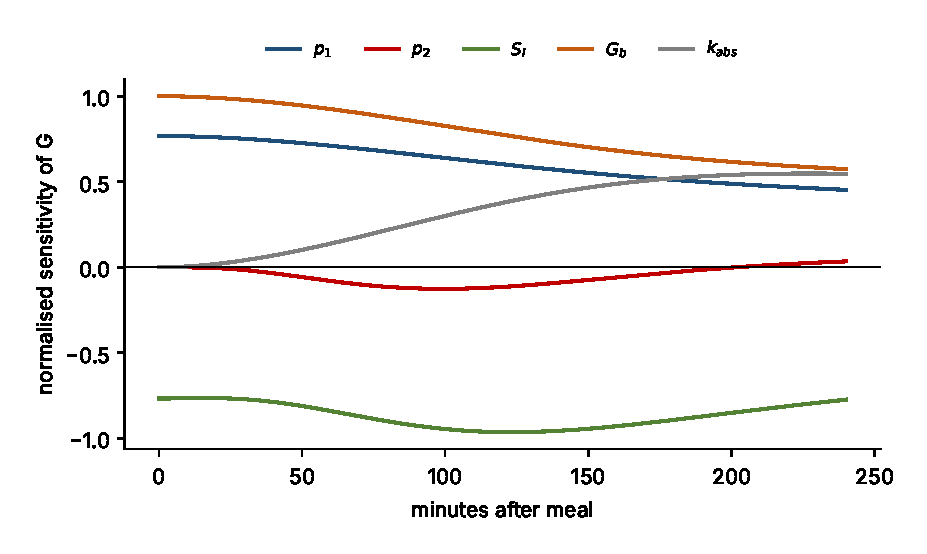
\includegraphics[width=0.49\textwidth]{local_sensitivity.eps}\hfill
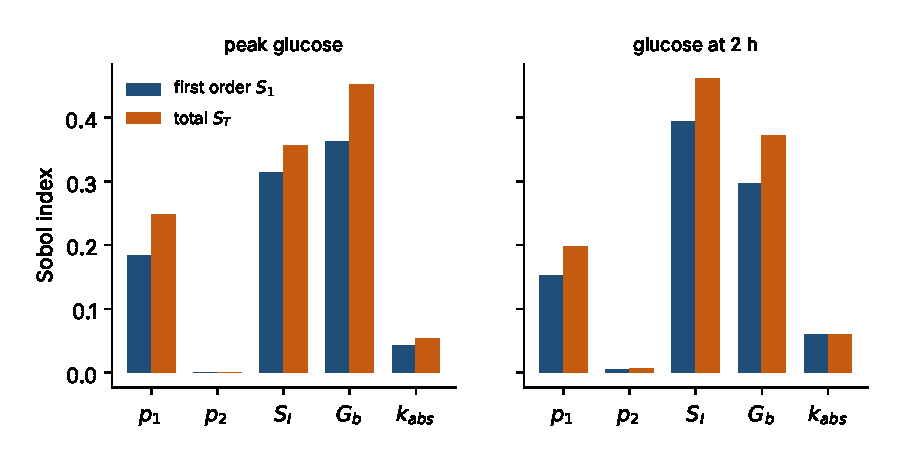
\includegraphics[width=0.49\textwidth]{sobol.eps}
\caption{Left: normalised local sensitivity of glucose after a meal. Right: first-order ($S_1$) and total ($S_T$) Sobol indices for peak glucose and glucose 2\,h after the meal.}
\label{fig:sens}
\end{figure}
\begin{table}[H]
\centering
\caption{Sobol indices (first order $S_1$, total $S_T$) for the reference patient, parameters varied in $[\theta/2, 2\theta]$.}
\label{tab:sobol}
\small
\begin{tabular}{lrrrr}
\toprule
 & peak glucose: $S_{1}$ & peak glucose: $S_{T}$ & glucose at 2 h: $S_{1}$ & glucose at 2 h: $S_{T}$ \\
\midrule
$p_1$ & 0.183 & 0.249 & 0.152 & 0.198 \\
$p_2$ & -0.000 & 0.000 & 0.004 & 0.007 \\
$S_I$ & 0.314 & 0.356 & 0.394 & 0.461 \\
$G_b$ & 0.363 & 0.453 & 0.297 & 0.372 \\
$k_{abs}$ & 0.042 & 0.054 & 0.060 & 0.060 \\
\bottomrule
\end{tabular}
\end{table}


\section{Numerical method and convergence}
Insulin \eqref{eq:insulin} does not depend on glucose, so $I(t)$ is computed once over each patient's whole record. The insulin action at the start of a window follows from the exact solution $X(t)=p_2S_I\int_0^\infty e^{-p_2 s}I(t-s)\,ds$ (24 h of history). Inside each window, $(Q_1,Q_2,X,G)$ are integrated by explicit Euler with $\Delta t=1$\,min; all rates are below 0.3\,min$^{-1}$, well inside the stability limit $\Delta t<2/|\lambda|$. Against an RK45 reference solution (tolerance $10^{-10}$), the error in glucose 4\,h after a meal halves each time $\Delta t$ halves (Table~\ref{tab:conv}, Figure~\ref{fig:conv}): observed order 1.19 (successive error ratios approach 2), as expected for a first-order method. At $\Delta t=1$\,min the error is 0.013\,mg/dL, negligible compared with CGM noise.

\begin{minipage}{0.48\textwidth}
\centering
\captionof{table}{Euler error in $G$ at 4\,h vs.\ RK45 reference.}\label{tab:conv}
\small
\begin{tabular}{rrl}
\toprule
$\Delta t$ (min) & error (mg/dL) & ratio \\
\midrule
8 & 0.1989 & 2.77 \\
4 & 0.0717 & 2.41 \\
2 & 0.0297 & 2.22 \\
1 & 0.0134 & 2.13 \\
0.5 & 0.0063 & 2.03 \\
0.25 & 0.0031 &  \\
\bottomrule
\end{tabular}

\end{minipage}\hfill
\begin{minipage}{0.48\textwidth}
\centering
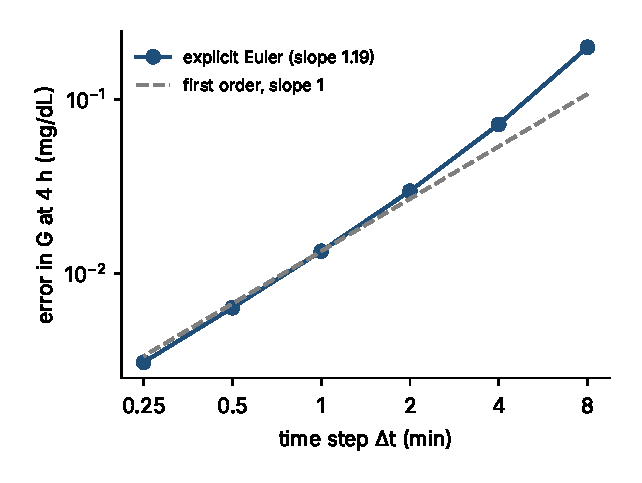
\includegraphics[width=\textwidth]{convergence.eps}
\captionof{figure}{Euler error vs.\ step size (log--log).}
\label{fig:conv}
\end{minipage}

\section{Extension: hybrid universal differential equation}
\paragraph{Motivation.} The fitted models and the sensitivity analysis point at the gut. Real meals raise glucose within 30--60 minutes and then fall, while the linear gut \eqref{eq:gut} with a single rate makes one smooth, slow bump; for many patients the fitted $k_{abs}$ sits at its lower bound. Physiologically, gastric emptying is nonlinear: it slows while the stomach is full and speeds up as it empties \cite{dallaman2007}.

\paragraph{Model.} We keep \eqref{eq:insulin} and \eqref{eq:bergman} and replace only the gut transfer rates by neural networks of the compartment contents:
\begin{equation}
\dot Q_1 = D\,\delta(t-t_m) - k_{abs}h_1(Q_1)Q_1,\quad \dot Q_2 = k_{abs}h_1(Q_1)Q_1 - k_{abs}h_2(Q_2)Q_2,\quad R_a=\frac{f\,k_{abs}h_2(Q_2)Q_2}{BW},
\end{equation}
\begin{equation}
h_i(q) = \exp\!\big(\ln 5\cdot\tanh(\mathrm{NN}_i(q/50\,\mathrm g))\big)\in[1/5,\,5],
\end{equation}
where each $\mathrm{NN}_i$ is a fully connected network $1\to16\to16\to1$ with $\tanh$ activations (305 weights each). The design choices are deliberate:
\begin{itemize}
  \item \textbf{Mass conservation:} each flux is a non-negative rate times the compartment content, so carbohydrate is never created or lost, and contents stay non-negative.
  \item \textbf{Nested models:} the networks' last layer is initialised to zero, so $h_i\equiv1$ and training starts exactly at the fitted Bergman model.
  \item \textbf{Shared physics, personal physiology:} $h_1,h_2$ are shared by all patients; $(p_1,p_2,S_I,G_b,k_{abs})$ remain patient-specific.
\end{itemize}

\paragraph{Training.} We use ``discretise-then-optimise'': the Euler solver is unrolled for all 240 one-minute steps, the masked MSE over training windows is computed, and gradients with respect to network weights and patient parameters are obtained by back-propagation through the solver (PyTorch autograd). Adam (learning rates $10^{-2}$ for the networks, $5\times10^{-3}$ for patient parameters) runs for up to 600 iterations, and the weights with the lowest validation RMSE are kept (early stopping). For unseen patients the networks are frozen and only their five parameters are fitted on their own training days.

\section{Validation on virtual patients (known truth)}
\subsection{Twin experiment: can a hidden mechanism be recovered?}
We generated synthetic CGM data from our own model --- same insulin records, meals, windows and fitted physiology as the real patients --- but with a \emph{nonlinear} stomach whose emptying saturates when full (Michaelis--Menten emptying, flux $V_{max}Q_1/(K_m+Q_1)$ with $V_{max}=0.4$\,g/min, $K_m=10$\,g, as in classic gastric-emptying models), a linear gut-to-blood rate of 0.05\,min$^{-1}$, and sensor noise of SD 5\,mg/dL. All other parts of the model are correct, so the question is clean: \emph{can the networks rediscover the emptying law from glucose readings alone?}

The answer is yes for what matters to glucose (Table~\ref{tab:sim}, Figure~\ref{fig:twin}): forecast RMSE on held-out meals falls from 14.4 to 6.1\,mg/dL, close to the noise level, and the error in the meal-appearance curve $R_a$ falls from 41\% to 7\%. The \emph{split} between the two gut stages is not recovered: two stages in series can trade speed and still produce the same $R_a$, so only their composite is identifiable from glucose.

\begin{figure}[H]
\centering
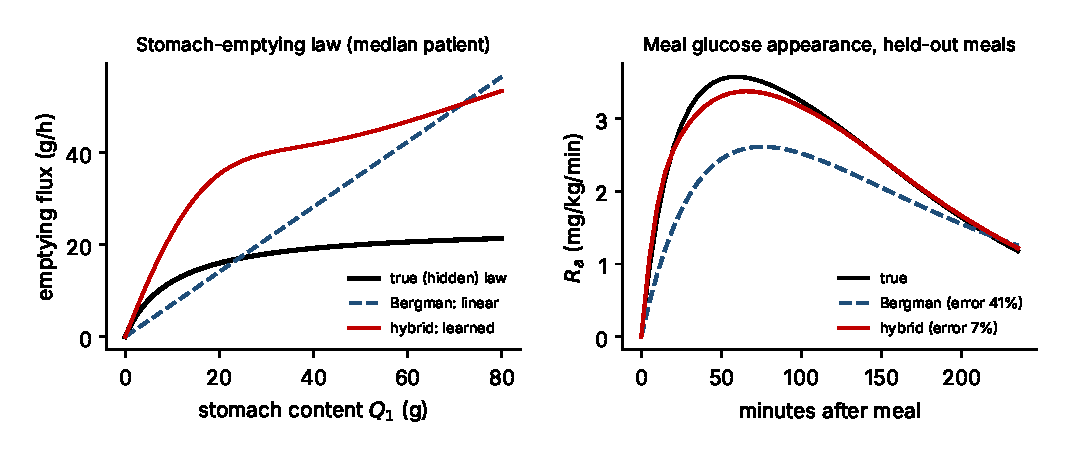
\includegraphics[width=\textwidth]{twin_recovery.eps}
\caption{Twin experiment, held-out meals. Left: stomach-emptying flux --- the hidden true law, the linear Bergman fit, and the hybrid's learned (saturating) law. Right: mean rate of glucose appearance $R_a$; the hybrid recovers the true curve (7\% error vs.\ 41\%).}
\label{fig:twin}
\end{figure}

\subsection{UVA/Padova virtual patients: a realistic, misspecified test}
Data from the UVA/Padova simulator come from a different, richer model (13 states, nonlinear gastric emptying depending on meal size, different insulin and glucose kinetics). Here the Bergman model is already accurate (RMSE 10.9\,mg/dL) and the hybrid improves it modestly (10.2\,mg/dL overall; 14.9 $\to$ 12.2\,mg/dL at 30\,min). However, its learned absorption profile is \emph{not} closer to the simulator's true one (Figure~\ref{fig:sim}): when other parts of the model are also wrong, the network improves forecasts by compensating for them rather than by identifying the gut. Better prediction does not by itself prove a recovered mechanism.

\begin{table}[H]
\centering
\caption{Forecast error (mg/dL) on held-out meals of synthetic patients. RMSE at 30\,min, 1, 2 and 4\,h after the meal, and over the whole window.}
\label{tab:sim}
\small
\begin{tabular}{llrrrrrr}
\toprule
 &  & 30 min & 1 h & 2 h & 4 h & RMSE all & MAE all \\
\midrule
\multirow[t]{3}{*}{Twin experiment} & Persistence & 33.5 & 67.4 & 102.4 & 111.8 & 90.0 & 73.0 \\
 & Bergman (mechanistic) & 8.6 & 13.6 & 14.3 & 22.0 & 14.4 & 9.7 \\
 & Hybrid UDE & 5.1 & 5.9 & 5.4 & 7.5 & 6.1 & 4.6 \\
\cline{1-8}
\multirow[t]{3}{*}{UVA/Padova} & Persistence & 15.2 & 44.0 & 37.8 & 24.3 & 32.1 & 25.1 \\
 & Bergman (mechanistic) & 14.9 & 13.9 & 9.8 & 11.3 & 10.9 & 8.0 \\
 & Hybrid UDE & 12.2 & 12.8 & 9.7 & 10.1 & 10.2 & 7.5 \\
\cline{1-8}
\bottomrule
\end{tabular}
\end{table}


\begin{figure}[H]
\centering
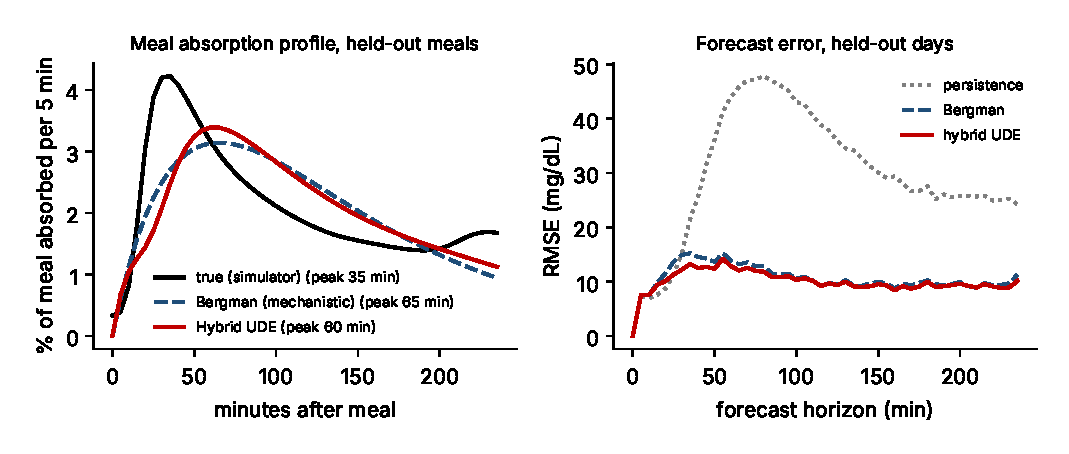
\includegraphics[width=\textwidth]{sim_validation.eps}
\caption{Virtual patients, held-out meals. Left: average meal absorption profile (fraction of the meal appearing in blood per 5 minutes) --- true simulator value vs.\ the mechanistic and hybrid models. Right: forecast RMSE against horizon.}
\label{fig:sim}
\end{figure}

\section{Results on real patients}
Table~\ref{tab:real} and Figure~\ref{fig:real} compare the four forecasters on held-out days. For patients seen in training, the two ODE models beat both baselines at every horizon: the hybrid UDE has the lowest error (42.7\,mg/dL), slightly ahead of Bergman (43.1), and well ahead of the LSTM (48.5) and persistence (49.8) --- with about 640 network weights against the LSTM's 51\,500. For the 4 patients never seen by the networks, the hybrid improves on Bergman by 8\% and ties the LSTM overall (56.2 vs 56.4). The LSTM, which sees two hours of glucose history, is best in the first hour; the hybrid is far better at 4\,h (62.9 vs 83.3\,mg/dL), where physiology matters more than the recent trend. The learned gut factors (Figure~\ref{fig:gut}) say that real meals empty from the stomach faster than the fitted linear model allows, and that the last part of a meal is absorbed quickly --- consistent with the fast rise and fall seen in the CGM traces.

\begin{table}[H]
\centering
\caption{Forecast error (mg/dL) on held-out days of real patients.}
\label{tab:real}
\small
\begin{tabular}{llrrrrrr}
\toprule
 &  & 30 min & 1 h & 2 h & 4 h & RMSE all & MAE all \\
\midrule
\multirow[t]{4}{*}{seen patients} & Persistence & 29.9 & 48.7 & 55.6 & 52.9 & 49.8 & 36.6 \\
 & Bergman (mechanistic) & 28.1 & 45.0 & 46.8 & 45.5 & 43.1 & 32.7 \\
 & Hybrid UDE & 27.9 & 44.8 & 46.0 & 43.0 & 42.7 & 32.3 \\
 & LSTM & 33.7 & 49.7 & 55.2 & 47.6 & 48.5 & 37.0 \\
\cline{1-8}
\multirow[t]{4}{*}{unseen patients} & Persistence & 26.5 & 36.3 & 69.6 & 86.9 & 61.6 & 44.5 \\
 & Bergman (mechanistic) & 42.7 & 53.2 & 73.3 & 66.4 & 61.2 & 45.3 \\
 & Hybrid UDE & 34.8 & 46.0 & 68.4 & 62.9 & 56.2 & 42.5 \\
 & LSTM & 22.5 & 30.3 & 62.1 & 83.3 & 56.4 & 41.3 \\
\cline{1-8}
\bottomrule
\end{tabular}
\end{table}


\begin{figure}[H]
\centering
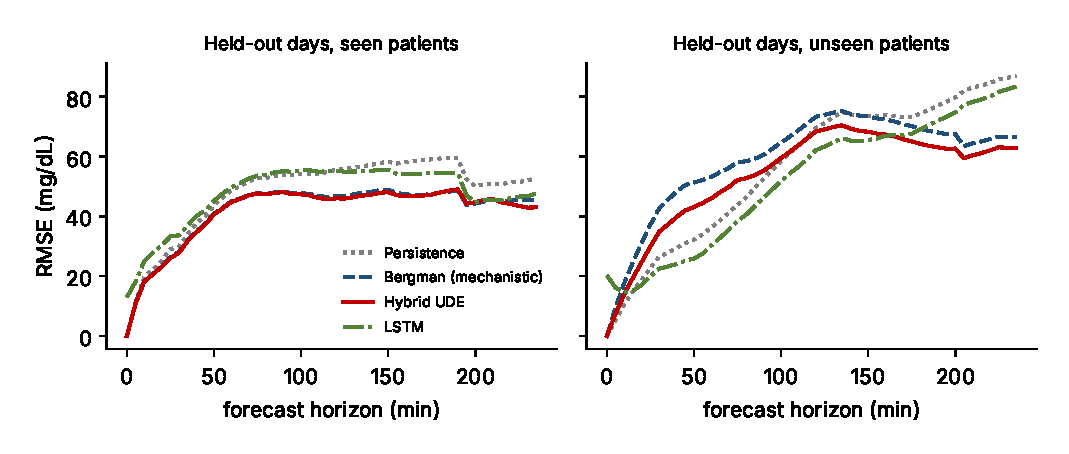
\includegraphics[width=\textwidth]{rmse_horizon_real.eps}
\caption{Forecast RMSE against horizon on held-out days, for patients seen in training (left) and never seen by the networks (right).}
\label{fig:real}
\end{figure}

\begin{figure}[H]
\centering
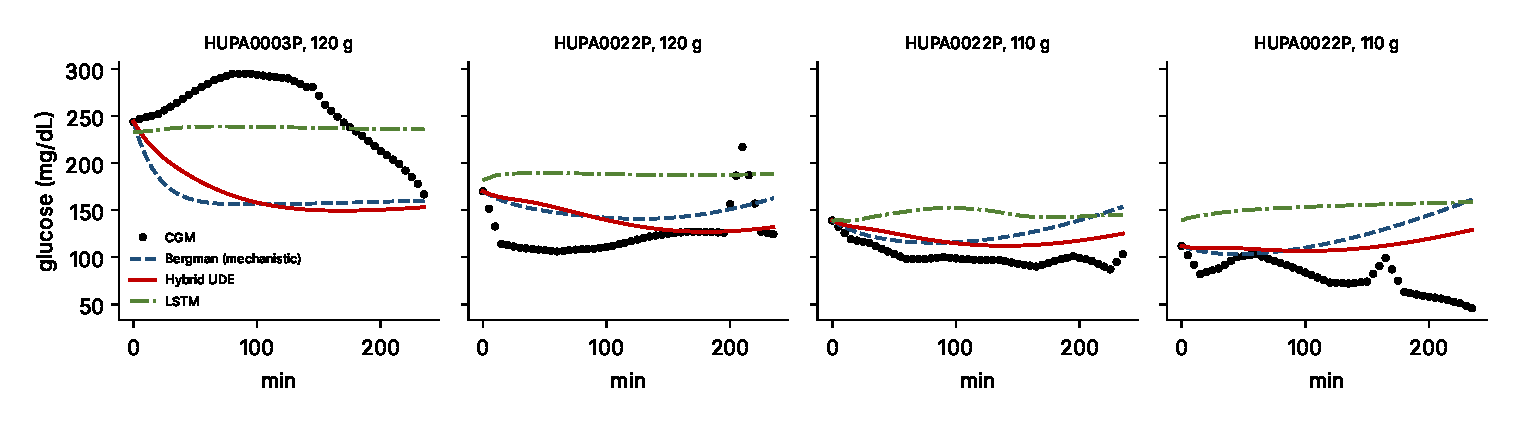
\includegraphics[width=\textwidth]{example_forecasts.eps}
\caption{Four held-out meals: CGM readings and 4-hour forecasts made at meal time.}
\label{fig:examples}
\end{figure}

\begin{figure}[H]
\centering
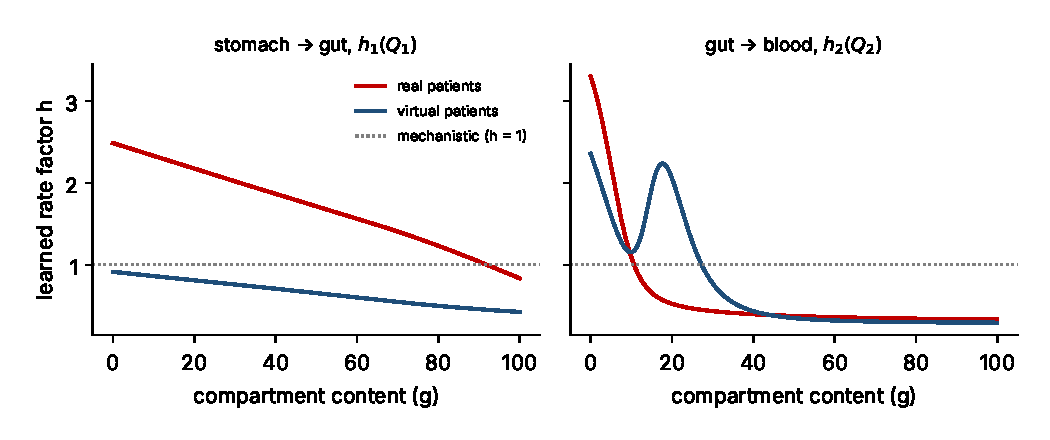
\includegraphics[width=0.9\textwidth]{learned_gut.eps}
\caption{Learned gut rate factors $h_1(Q_1)$, $h_2(Q_2)$; $h=1$ is the mechanistic model.}
\label{fig:gut}
\end{figure}

\section{Discussion and limitations}
The three tests tell a consistent story. When the rest of the model is right (twin experiment), a small, mass-conserving network inside the ODE recovers an unknown physiological law and cuts forecast error by more than half. When the rest of the model is also approximate (simulator and real patients), the same network still improves forecasts --- most clearly for patients it never saw --- but its learned shape should be read as a correction that compensates for several model errors, not as a measurement of gastric emptying. On real data the dominant error is not the model structure but missing information: unlogged meals and exercise. This is why all four methods, including a much larger LSTM, have similar and large errors, and why the physiology-based models --- which encode how insulin and carbohydrate act --- generalise better than the purely data-driven one beyond the first hour.

\paragraph{Limitations.}
\begin{itemize}
  \item \textbf{Unlogged events:} about half of all boluses have no logged meal nearby; snacks, exercise and stress are invisible to all models and dominate the real-data error (Figure~\ref{fig:data}).
  \item \textbf{Carbohydrate counts} are patient estimates, typically wrong by 20--50\%, and most patients log in 10\,g portions.
  \item \textbf{CGM} measures interstitial glucose with a 5--10 minute lag and is a 15-minute sensor interpolated to 5 minutes.
  \item \textbf{Unknown body weight} and weak identifiability mean the fitted parameter values should not be compared with clinical studies; some patients' fitted $G^*$ are unphysiological.
  \item \textbf{Small data:} 15 patients and about 300 training meals; the unseen-patient test has only 30 meals.
\end{itemize}

\begin{figure}[H]
\centering
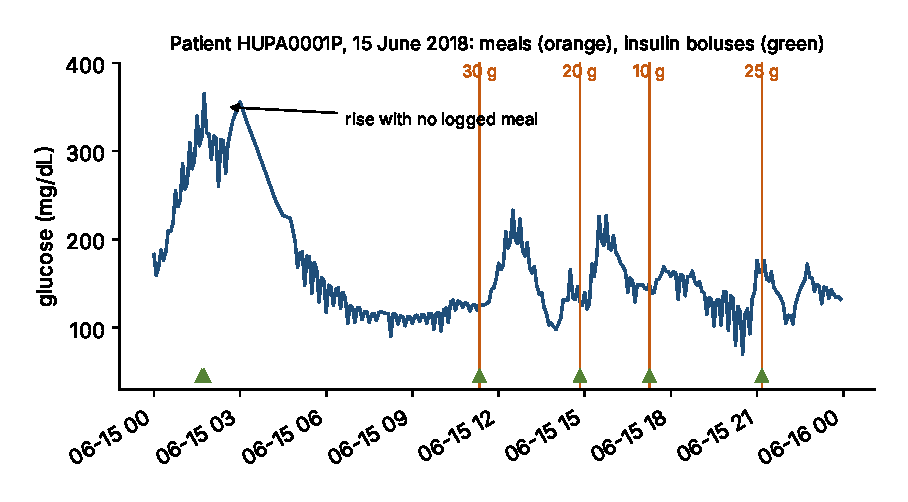
\includegraphics[width=0.75\textwidth]{data_one_day.eps}
\caption{One day of real data (patient HUPA0001P): glucose rises sharply around 02:00 with no logged meal.}
\label{fig:data}
\end{figure}

\paragraph{Extensions.} Model the CGM sensor lag; treat unlogged meals as latent inputs estimated with a Kalman or particle filter; add a learned residual for exercise using the heart-rate and step data already in the dataset.

\section{Conclusion}
We adapted the Bergman minimal model to Type 1 diabetes, proved that its basal equilibrium is a unique, stable node with fasting glucose $G^*=p_1G_b/(p_1+S_II^*)$, identified which parameters the data can and cannot determine, and showed with Sobol analysis that insulin sensitivity and $G_b$ dominate the meal response. Embedding small mass-conserving neural networks in the gut gave a hybrid universal differential equation that recovers a hidden absorption law in a controlled test, and on real patients matches or beats both the mechanistic model and an LSTM, especially for unseen patients and long horizons, while remaining interpretable. The main obstacle to accurate real-world forecasting is unrecorded behaviour, which future work should model as latent inputs.

\section*{Acknowledgement of AI tools}
Claude (Anthropic, accessed through claude.ai) was used to locate public datasets, suggest the model structure, analysis and validation design, write and debug Python code for the notebook, and draft and typeset this report. All equations, code and results were checked, run and edited by the group, and every member can explain them.

\begin{thebibliography}{99}
\bibitem{bergman1979} R.~N. Bergman, Y.~Z. Ider, C.~R. Bowden, C.~Cobelli. Quantitative estimation of insulin sensitivity. \emph{American Journal of Physiology} 236(6):E667--E677, 1979.
\bibitem{hovorka2004} R.~Hovorka et al. Nonlinear model predictive control of glucose concentration in subjects with type 1 diabetes. \emph{Physiological Measurement} 25(4):905--920, 2004.
\bibitem{dallaman2007} C.~Dalla Man, R.~A. Rizza, C.~Cobelli. Meal simulation model of the glucose--insulin system. \emph{IEEE Transactions on Biomedical Engineering} 54(10):1740--1749, 2007.
\bibitem{kovatchev2009} B.~P. Kovatchev, M.~Breton, C.~Dalla Man, C.~Cobelli. In silico preclinical trials: a proof of concept in closed-loop control of type 1 diabetes. \emph{Journal of Diabetes Science and Technology} 3(1):44--55, 2009.
\bibitem{hupa2024} J.~I. Hidalgo, J.~Alvarado, M.~Botella, A.~Aramendi, J.~M. Velasco, O.~Garnica. HUPA-UCM diabetes dataset. \emph{Data in Brief} 55:110559, 2024. Data: \url{https://data.mendeley.com/datasets/3hbcscwz44/1}.
\bibitem{simglucose} J.~Xie. Simglucose v0.2.1: a Type-1 diabetes simulator implemented in Python, 2018. \url{https://github.com/jxx123/simglucose}.
\bibitem{rackauckas2020} C.~Rackauckas et al. Universal differential equations for scientific machine learning. arXiv:2001.04385, 2020.
\bibitem{chen2018} R.~T.~Q. Chen, Y.~Rubanova, J.~Bettencourt, D.~Duvenaud. Neural ordinary differential equations. \emph{NeurIPS} 2018.
\bibitem{saltelli2002} A.~Saltelli. Making best use of model evaluations to compute sensitivity indices. \emph{Computer Physics Communications} 145(2):280--297, 2002.
\bibitem{salib} J.~Herman, W.~Usher. SALib: an open-source Python library for sensitivity analysis. \emph{Journal of Open Source Software} 2(9):97, 2017.
\bibitem{lstm} S.~Hochreiter, J.~Schmidhuber. Long short-term memory. \emph{Neural Computation} 9(8):1735--1780, 1997.
\end{thebibliography}

\end{document}
